% Load preamble
\documentclass[../main.tex]{subfiles}

\begin{document}

\subsection{Stavový opis}
Stavový opis je jedna z foriem opisu dynamického lineárneho systému. Základom je definovanie vnútorných stavov systému, ako sa tieto stavy menia v čase a ako vyzerá výstup zo systému.
\begin{equation}
	\begin{aligned}
        \dot{x} &= Ax + Bu \\
        y &= Cx + Du
	\end{aligned}
	\label{eqn:matz_stavovaRovnica}
\end{equation}

Pre SISO systémy je C vektor (riadkový) a D skalár. Pre MIMO systémy je C matica a D je vektor (stĺpcový). Majme systém opísaný rovnicami \ref{eqn:matz_system}.
\begin{equation}
	\begin{split}
        \dot{x_1} &= x_2 \\
		\dot{x_2} &= x_3 \\
		\dot{x_3} &= -x_1 + 8x_2 + 3x_3 - 6u \\
        y &= x_1
	\end{split}
	\label{eqn:matz_system}
\end{equation}
Tento systém môžeme napísať aj v maticovom tvare:
        \begin{center}
		$\begin{bmatrix} 
			\dot{x_1} \\ 
			\dot{x_2} \\ 
			\dot{x_3} \\ 
		\end{bmatrix}  = 
		\begin{bmatrix} 
			0 & 1 & 0 \\ 
			0 & 0 & 1 \\ 
			-1 & 8 & 3 \\ 
		\end{bmatrix} 
		\begin{bmatrix} 
			x_1 \\ 
			x_2 \\ 
			x_3 \\ 
		\end{bmatrix} +
		\begin{bmatrix} 
			0 \\ 
			0 \\ 
			-6 \\ 
		\end{bmatrix}
		u $
	\label{eqn:matz_system2}
        \end{center}

        \begin{center}
		$y  = 
		\begin{bmatrix} 
			1 & 0 & 0 \\ 
		\end{bmatrix} 
		\begin{bmatrix} 
			x_1 \\ 
			x_2 \\ 
			x_3 \\ 
		\end{bmatrix} +
		0u $
	\label{eqn:matz_system2}
        \end{center}
Laplaceovou transformáciou získame rovnice \ref{eqn:matz_systemLap}. 
\begin{equation}
	\begin{aligned}
		Ys^3 = -Y + 8 Ys + 3Ys^2 - 6U
	\end{aligned}
	\label{eqn:matz_systemLap}
\end{equation}
\begin{equation}
	\begin{aligned}
		Y(s^3 -3s^2 -8s + 1) = - 6U
	\end{aligned}
\end{equation}
\begin{equation}
	\begin{aligned}
		\frac{Y}{U} = \frac{-6}{s^3 -3s^2 -8s + 1} = G(s)
	\end{aligned}
	\label{eqn:matz_systemPrenos}
\end{equation}
kde rovnica  \ref{eqn:matz_systemPrenos} predstavuje prenosovú funkciu nášho systému.

Simulačná schéma je na obr. \ref{fig:matz_systemStavovyOpisSimulink}. V bloku integrátor je možné nastaviť počiatočné hodnoty stavov (počiatočné podmienky). Pri tejto schéme je dôležité uvedomiť si dimenzie (rozmer, či je to matica, vektor alebo skalár) jednotlivých signálov.
\begin{figure}[h!]
	\centering
	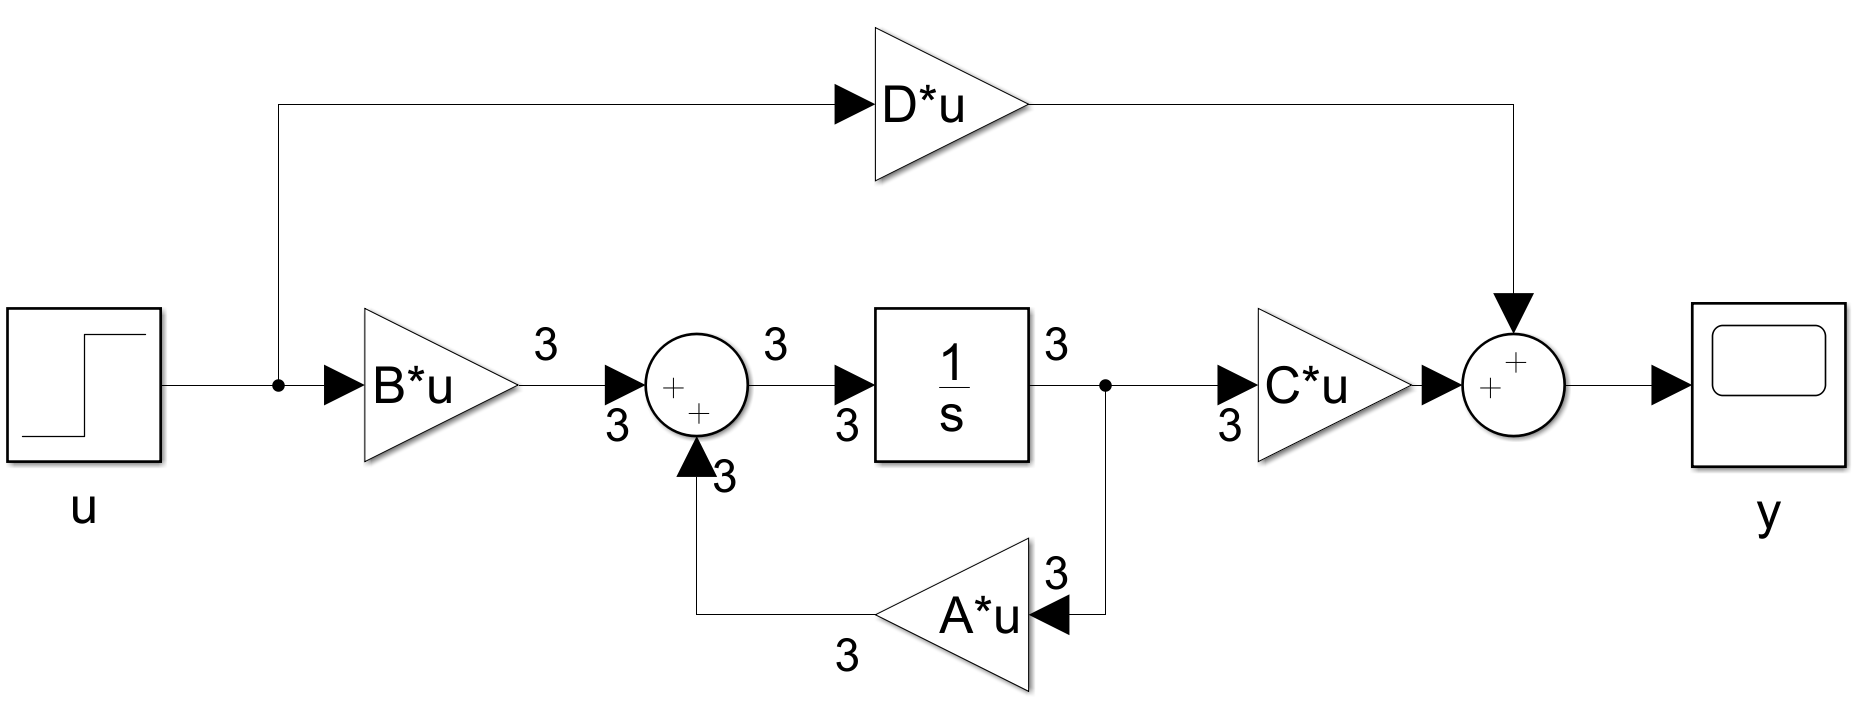
\includegraphics[width=0.8\linewidth]{matzaklady/SchemaStavovyOpis}
	\caption{Simulačná schéma systému definovaná pomocou stavového opisu}
	\label{fig:matz_systemStavovyOpisSimulink}
\end{figure}

\subsection{Rovnovážne stavy}
Rovnovážny stav $\dot{x_r}$ systému je definovaný ako stav, kedy sa stavové premenné nelineárneho systému nemenia v čase. 

V rovnovážnom stave platí pre vstup $u$, že je v každom čase nulový, $u(t)=0$. Pre stavove premenné platí $\dot{x}|_{x = x_r} = 0$.

Uvažujme príklad \ref{eqn:matz_system} a nájdime jeho rovnovážne stavy. Ako prvé položíme všetky derivácie (označené bodkami nad premennými v stavovom opise) rovné 0 ($\dot{x_1} = 0,\dot{x_2} = 0,\dot{x_3} = 0$). Dostaneme tak sústavu \ref{eqn:rovnovazny_stav1}.
\begin{equation}
	\begin{aligned}
        0 &= x_2 \\
		0 &= x_3 \\
		0 &= -x_1 + 8x_2 + 3x_3\\
	\end{aligned}
	\label{eqn:rovnovazny_stav1}
\end{equation}
hodnoty $x_2$ a $x_3$ vieme priamo vyčítať z rovnice vyššie, majú byť $x_2=0$ a $x_3=0$. Hodnotu $x_1$ musíme vypočítať. Našťastie, pre tento jednoduchý prípad, stačí dosadiť $x_2=0$ a $x_3=0$ do tretej rovnice sústavy \ref{eqn:rovnovazny_stav1} a dostaneme $x_1=0$.

Bod $[x_{r1},x_{r2},x_{r3}] = [0,0,0]$ je riešením sústavy rovníc \ref{eqn:rovnovazny_stav1}, preto je rovnovážnym stavom systému rovníc \ref{eqn:matz_system}.

Uvažujme teraz systém opisaný rovnicami \ref{eqn:rovnovazny_stav2} a nájdime jeho rovnovážne stavy.
\begin{equation}
	\begin{aligned}
        \dot{x_1} &= x_2 \\
		\dot{x_2} &= -\frac{b}{m}x_2-\frac{g}{L}sin(x_1) \\
	\end{aligned}
	\label{eqn:rovnovazny_stav2}
\end{equation}
Položíme derivácie rovné nule, z čoho dostaneme sútavu \ref{eqn:rovnovazny_stav22}.
\begin{equation}
	\begin{aligned}
        0 &= x_2 \\
		0 &= -\frac{g}{L}sin(x_1) \implies sin(x_1) = 0\\
	\end{aligned}
	\label{eqn:rovnovazny_stav22}
\end{equation}
Riešení sútavy \ref{eqn:rovnovazny_stav22} je niekoľko. Rovnovážnym bodom je nielen bod $[x_{r1},x_{r2}] = [0,0]$, ale všetky body $[x_{r1},x_{r2}] = [k*\pi,0],k \in Z$, kde $k \in Z$ znamená, že $k$ je z množiny $Z$, kde $Z$ je množina celých čísel, teda, že $k$ je celé číslo.
	
\subsection{Linearizácia}
Linearizácia je proces, pri ktorom z nelineárneho systému spravíme lineárny. Tento lineárny systém opisuje pôvodný systém "presne" len v okolí pracovného bodu. Veľkosť tohto okolia záleží od priebehu funkcií. Používa sa pri tom rozvoj do Taylorovho radu (rovnica \ref{fig:matz_systemStavovyOpisSimulink}), kedy použijeme len prvý člen.

\begin{equation}
	\begin{aligned}
		f(x) = \sum^{inf}_{n=0}{\frac{f^{(n)}(a)}{n!}(x-a)^n}
	\end{aligned}
	\label{eqn:matz_taylorovRad}
\end{equation}
kde $f^{(n)}$ je $n$-tá derivácia funkcie $f$ v bode $a$, v prípade funkcie viacerých premenných je to gradient. Funkcia $f$ musí byť diferencovatelná.

Pri linearizácií pôvodná nelineárna funkcia nahradí prvý člen Taylorovho radu (ostatné členy členy niesú linearárne, pretože majú faktor $(x-a)^n$ s $n > 1$), ktorý je daný \ref{eqn:matz_prvyClenTaylorovhoRadu}.
\begin{equation}
	\begin{aligned}
		f(x) \approx \frac{f^{(1)}(x)}{1!}(x-x_0)^1 = \frac{\partial{f}}{\partial{x}}|_{a}(x-x_0) = \nabla{f}|_{a}\Delta{x}
	\end{aligned}
	\label{eqn:matz_prvyClenTaylorovhoRadu}
\end{equation}

Majme systém opísaný rovnicami \ref{eqn:matz_rovniceSystemu}.
\begin{center}
$x = \begin{bmatrix}
\Delta{x_1} \\
\Delta{x_2} \\
\Delta{x_3} \\
\Delta{u}
\end{bmatrix}$
\end{center}
\begin{equation}
		\begin{aligned}
		\dot{x_1} &= x_1 + x_2 - x_3 + sin(x_2) 			\\
		\dot{x_2} &= - x_1 - x_2 						\\
		\dot{x_3} &= cos(x_2) (sin(x_2) - x_3) - u 	\\
		y &= x_1
		\end{aligned}
		\label{eqn:matz_rovniceSystemu}
\end{equation}

Keďže sa v sústave \ref{eqn:matz_rovniceSystemu} vyskytujú aj nelineárne členy (všetko čo nieje konštanta po derivácii je nelineárne, napríklad: sínus, kosínus a ich súčin), tento systém je nelineárny. 

% Toto mi nedáva zmysel
Pri linearizácií tohto systému musíme počítať gradient každej rovnice podľa stavového vektora a vstupov, ďalej len vektora parametrov funkcií $x$. Nech bod P [0 0 0 0] je pracovným bodom, v ktorom budeme systém linearizovať.

\begin{equation}
		\begin{aligned}
		\nabla{\dot{x_1}} &= [\frac{\partial{\dot{x_1}}}{\partial{x_1}},\frac{\partial{\dot{x_1}}}{\partial{x_2}},\frac{\partial{\dot{x_1}}}{\partial{x_3}},\frac{\partial{\dot{x_1}}}{\partial{u}}] = [1, 1 + cos(x_2), -1, 0]			\\
		\nabla{\dot{x_2}} &= [\frac{\partial{\dot{x_2}}}{\partial{x_1}},\frac{\partial{\dot{x_2}}}{\partial{x_2}},\frac{\partial{\dot{x_2}}}{\partial{x_3}},\frac{\partial{\dot{x_2}}}{\partial{u}}] = [-1, -1, 0, 0]			\\
		\nabla{\dot{x_3}} &= [\frac{\partial{\dot{x_3}}}{\partial{x_1}},\frac{\partial{\dot{x_3}}}{\partial{x_2}},\frac{\partial{\dot{x_3}}}{\partial{x_3}},\frac{\partial{\dot{x_3}}}{\partial{u}}] = [0, -sin^2(x_2)+cos^2(x_2), -cos(x_2), -1]			\\
		y &= [\frac{\partial{y}}{\partial{x_1}},\frac{\partial{y}}{\partial{x_2}},\frac{\partial{y}}{\partial{x_3}},\frac{\partial{y}}{\partial{u}}] = [1, 0, 0, 0]			\\
		\end{aligned}
		\label{eqn:matz_rovniceSystemuGradient}
\end{equation}
Gradient v pracovnom bode dostaneme dosadením hodnôt pracovného bodu.
\begin{equation}
		\begin{aligned}
		\nabla{\dot{x_1}}|_{P} &= [1, 1 + cos(0), -1, 0] = [1, 2, -1, 0]			\\
		\nabla{\dot{x_2}}|_{P} &= [-1, -1, 0, 0] \\
		\nabla{\dot{x_3}}|_{P} &= [0, -sin^2(0)+cos^2(0), -cos(0), -1] = [0,1, -1, -1]			\\
		\nabla{y}|_{P} &= [1, 0, 0, 0]			\\
		\end{aligned}
		\label{eqn:matz_rovniceSystemuGradient}
\end{equation}
Ak vynásobíme gradienty v pracovnom bode vektorom $x$, dostaneme linearizovanú sústavu diferenciálnych rovníc, ktoré opisujú správanie sa systému v okolí pracovného bodu $P$, rovnice \ref{eqn:matz_rovniceLinearnySystem}.
\begin{equation}
		\begin{aligned}
		\Delta{\dot{x_1}} &= \Delta{x_1} + 2\Delta{x_2} - \Delta{x_3}			\\
		\Delta{\dot{x_2}} &= -\Delta{x_1} - \Delta{x_2} \\
		\Delta{\dot{x_3}} &= \Delta{x_2} - \Delta{x_3} - \Delta{u}		\\
		\Delta{y} &= \Delta{x_1}			\\
		\end{aligned}
		\label{eqn:matz_rovniceLinearnySystem}
\end{equation}
	
\subsection{Riešenie preurčenej sústavy rovníc}
Preurčená sústava rovníc, obsahuje viac rovníc ako neznámych premenných. Pri riešení preurčenej sústavy rovníc použijeme metódu najmenších štvorcov. Pomocou metódy najmenších štvorcov určíme riešenie preurčenej sústavy rovníc \ref{eqn:MaticovyZapisPSR} s najmenšou chybou.
\begin{equation}
    Ax = b 
	\label{eqn:MaticovyZapisPSR}
\end{equation}
Uvažujeme nasledovnú preurčenú sústavu rovníc:
\begin{equation}
	\begin{aligned}
	 x+y  & = 5 \\
	 2x+4y+10 & = 8 \\
	 x+5y & = 15 \\
	 -2x+4y+10 & = 8 \\
	\end{aligned}
	\label{eqn:PreurcenySystem}
\end{equation}
Preurčenú sústavu rovníc \ref{eqn:PreurcenySystem} môžeme maticovo zapísať v tvare:
\begin{equation}
    \begin{bmatrix} 1 & 1\\ 2 & 4 \\1 &5 \\-2& 4\end{bmatrix}\begin{bmatrix}x \\y \end{bmatrix} = \begin{bmatrix} 5 \\-2\\15\\-2 \end{bmatrix}
    \label{eqn:MaticovyZapisPiklad}
\end{equation}
Na výpočet neznámych premenných x,y použijeme metódu najmenších štvorcov:
\begin{equation}
	\begin{aligned}
	\begin{bmatrix}x \\y \end{bmatrix} &=  (A^TA)^{-1}A^Tb\\
	\begin{bmatrix}x \\y \end{bmatrix} &=  \begin{bmatrix} 1.4265 \\0.9559\end{bmatrix}
	\end{aligned}
	\label{eqn:MNS}
\end{equation}

\subsection{Parciálne derivácie}
Majme funkciu $f$ o viacerých premenných $f(x,y,z, ...)$. Parciálna derivácia funkcie $f$, je derivácia funkcie $f$ vzhľadom na 1 premennú, pričom o ostatných premenných uvažujeme ako o konštantách.

Parciálnu deriváciu budeme označovať $\frac{\partial f(x,y,z,\dots}{\partial x}$,$\frac{\partial f(x,y,z,\dots)}{\partial y}$,$\frac{\partial f(x,y,z,\dots)}{\partial z} \dots$.

Vypočítajme parciálne derivácie funkcie \ref{eqn:parcpr1}.
\begin{equation}
    \begin{aligned}
        f(x,y)= \frac{x}{x^2+y^2}
    \end{aligned}
    \label{eqn:parcpr1}
\end{equation}
pričom najskôr vypočítame parciálnu deriváciu podľa premennej $x$. Aplikujeme pravidlo o derivácií podielu dvoch funkcií $h,g$: $(\frac{h}{g})'= \frac{h'g-g'h}{g^2}$.
\begin{equation}
	\begin{aligned}
	\frac{\partial}{\partial x}\frac{x}{x^2+y^2} &= \frac{\frac{\partial x}{\partial x}(x^2+y^2)-\frac{\partial (x^2+y^2)}{\partial x}x}{(x^2+y^2)^2} \\
	&= \frac{1(x^2+y^2)-2xx}{(x^2+y^2)^2}\\
	&= \frac{-x^2+y^2}{(x^2+y^2)^2}\\
	\end{aligned}
	\label{eqn:PDx}
\end{equation}
Parciálna derivácia podľa premennej $y$ má nasledujúci tvar 
\begin{equation}
	\begin{aligned}
	\frac{\partial}{\partial y}\frac{x}{x^2+y^2} &= x\frac{\partial}{\partial y}\frac{1}{x^2+y^2} \\
	&= x\frac{\partial}{\partial y}(x^2+y^2)^{-1} \\
	&= x(x^2+y^2)^{-2}\frac{\partial}{\partial y}(x^2+y^2) \\
	&= \frac{2xy}{(x^2+y^2)^{2}} \\
	\end{aligned}
	\label{eqn:PDy}
\end{equation}
Ako druhú ukážku, parciálne derivácie funkcie danej ronvicou \ref{eqn:parcpr2}.
\begin{equation}
    \begin{aligned}
f(x,y)= sin(xy)+\frac{1}{2}cos(y)
    \end{aligned}
    \label{eqn:parcpr2}
\end{equation} 
pričom najskôr vypočítame parciálnu deriváciu podľa premennej $x$.
\begin{equation}
	\begin{aligned}
	\frac{\partial}{\partial x}(sin(xy)+\frac{1}{2}cos(y)) &= \frac{\partial}{\partial x}sin(xy)+\frac{\partial}{\partial x}\frac{1}{2}cos(y)) \\
	&= \frac{\partial}{\partial x}sin(xy)\frac{\partial}{\partial x}(xy)\\
	&= cos(xy)y \\
	\end{aligned}
	\label{eqn:PDx2}
\end{equation}
Parciálnu deriváciu podľa podľa premennej $y$ vieme vypočítať nasledovne:
\begin{equation}
	\begin{aligned}
	\frac{\partial}{\partial y}(sin(xy)+\frac{1}{2}cos(y)) &= \frac{\partial}{\partial y}sin(xy)+\frac{\partial}{\partial y}\frac{1}{2}cos(y)) \\
	&= \frac{\partial}{\partial y}sin(xy)\frac{\partial}{\partial y}(xy)-\frac{1}{2}sin(y)) \\
	&= cos(xy)x - \frac{1}{2}sin(y) \\
	\end{aligned}
	\label{eqn:PDy2}
\end{equation}
		
\end{document}
